\chapter{СВЕРТОЧНЫЕ НЕЙРОННЫЕ СЕТИ ДЛЯ ДЕТЕКТИРОВАНИЯ}

\section{Сверточные нейронные сети}

%Распознавание и классификация изображений достаточно успешно осуществляются с помощью сверточных нейронных сетей. Нейронная сеть – это некоторая математическая модель, которая состоит из соединенных между собой искусственных нейронов . Сеть принимает в качестве входных данных вектор признаков, затем последовательно пропускает их через слои сети. На выходе получаются вероятности принадлежности объекта к заданным классам. Обычно нейронная сеть оперирует числовыми, а не символьными величинами.

Сеть свертки представляет собой многoслойный персептрон -- математическая или компьютерная модель восприятия информации мозгом, созданный для распознавания 2D-поверхностей с высокой степенью устойчивости к масштабированию, преобразованиям и другим видам деформации. Обучение решению такой задачи осуществляется с подкреплением, при этом используются сети вида, архитектура которых соответствует следующим ограничениям .

Каждый нейрон получает входной сигнал от локального рецептивного поля в предыдущем слое, извлекая его локальные признаки. Как только признак извлечен, его местоположение не имеет значения, т.к. приблизительно установлено его расположение относительно других признаков.

Каждый вычислительный слой сети состоит из множества карт признаков. Каждая карта признаков имеет форму плоскости, на которой все нейроны должны совместно использовать одно и то же множество синаптических весов. Эта форма структурных ограничений имеет преимущества.

За каждым слоем свертки следует вычислительный слой, осуществляющий локальное усреднение (local averaging) и подвыборку (subsampling). Посредством локального усреднения достигается уменьшение разрешения для карт признаков. Такая операция приводит к уменьшению чувствительности выходного сигнала оператора отображения признаков, а также к смещению и другим формам преобразований.


\section{YOLO}

YOLO  – это свёрточная нейронная сеть, позволяющая детектировать и классифицировать объекты в виде обрамляющих прямоугольников. YOLO работает по принципу Single Shot. Это значит, что архитектура сети устроена таким образом, что за один проход кадра, на нём детектируются все объекты.

На рисунке \ref{img:yolo} представлена архитектура YOLO. На вход YOLO подается трёхканальное изображение, у которого меняется размер до 448x448, над полученным изображением проводятся преобразования. Первое преобразование заключается в прогоне изображения через часть модифицированной архитектуры GoogLeNet. После этого преобразования получается feature maps размером 14x14x1024. Далее применяются две конволюции. После второй конволюции размерность уменьшается до 7x7x1024. Далее проводится ещё одна конволюция. Результат дважды прогоняется через полносвязный слой, изменяется до размерности 1470x1 и в итоге трансформируется в тензор размером 7x7x30. К полученному тензору применяется процедура детектирования, на выходе которой получается результирующее детектирование. Тензор представляет собой отображение сетки 7x7 на изображении. 30 значений несут информацию о ячейке: 10 значений для двух возможных рамок, 20 значений отношения к каждому из 20 доступных классов. Вся эта информация фильтруется, отфильтрованные данные отображаются.


\begin{figure}[H]
\centering
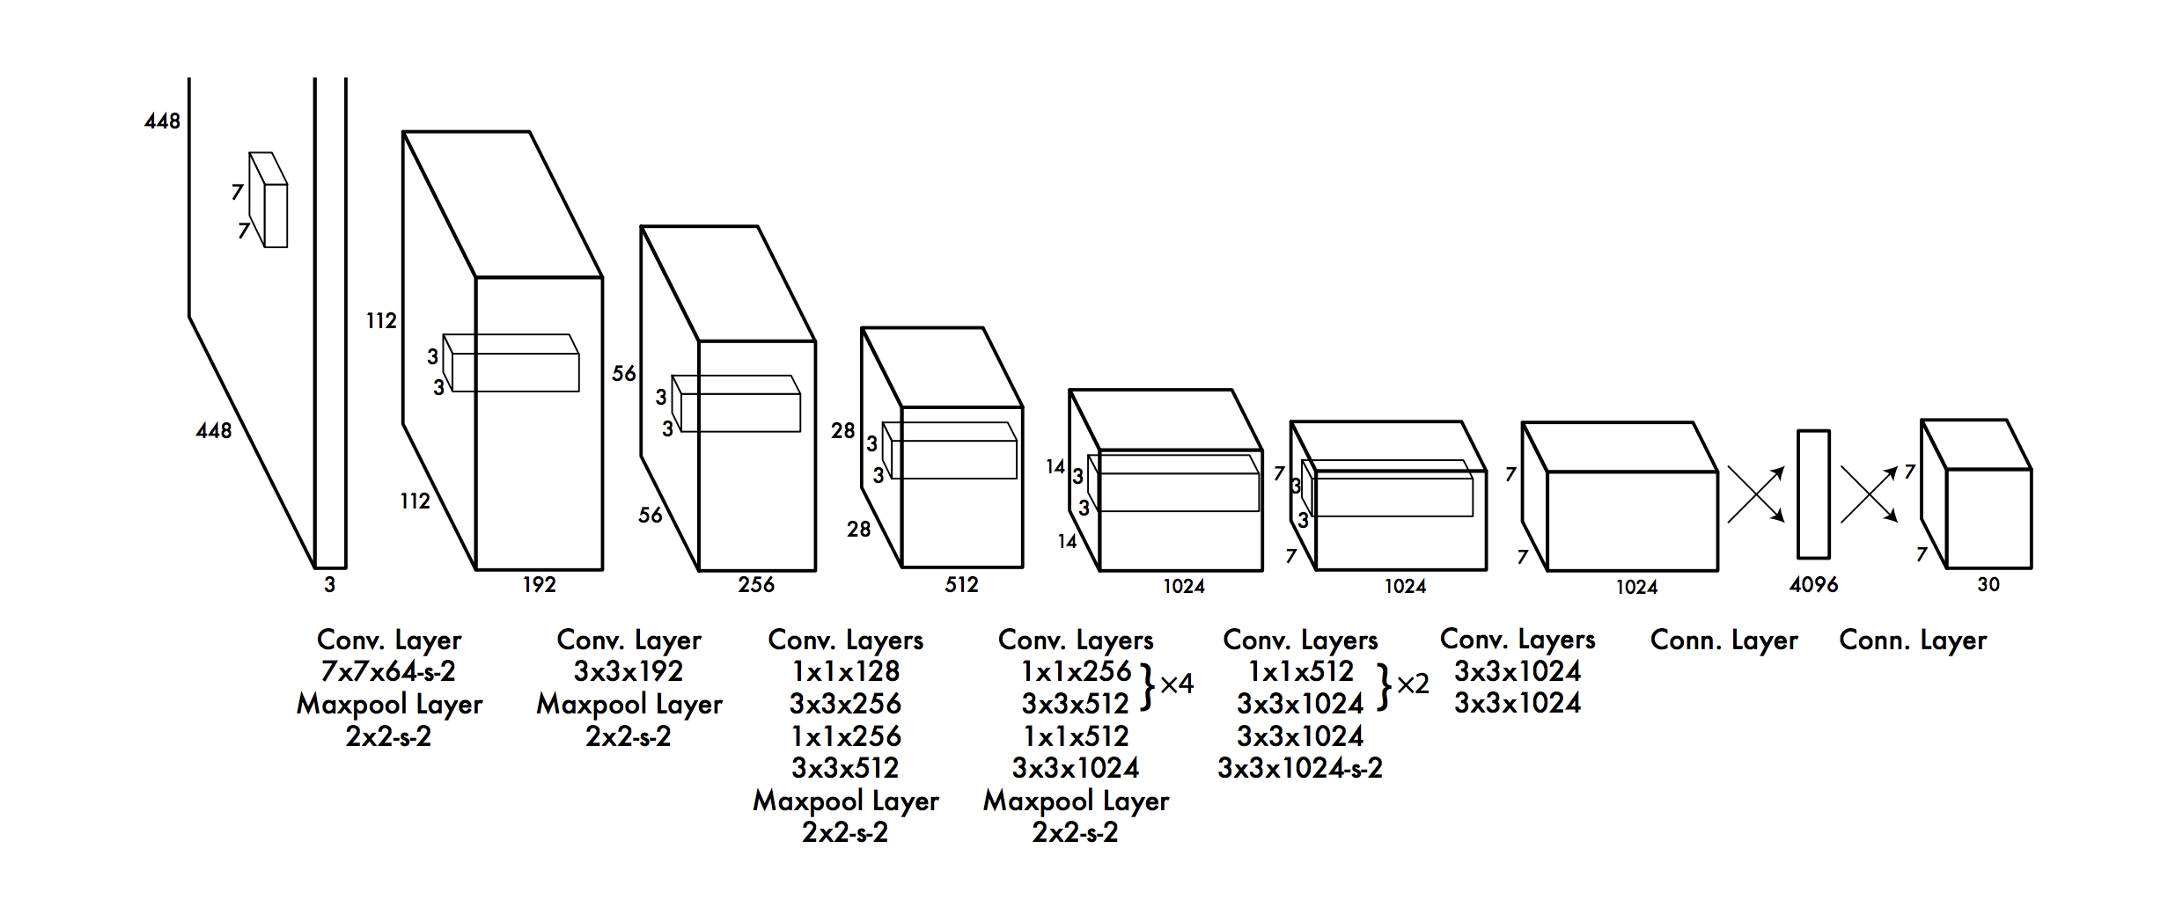
\includegraphics[width=15cm]{images/yolo.png}
\caption{Архитектура YOLO}
\label{img:yolo}
\end{figure}


\chapter{АРХИТЕКТУРА СИСТЕМЫ}


\section{Получение информации}


Система получает изображение с камеры видеонаблюдения. Предполагается, что камера установлена под некоторым фиксированным углом, а кадры выровнены в горизонтальной плоскости. 

\section{Калибровка}

Для вычисления расстояния нам необходимо сопоставить координаты на изображении и в реальном мире. Для этого мы используем инструмент калибровки.


В процессе калибровки мы запрашиваем у пользователя координаты квадрата на изображении, все точки которого располагаются на плоскости, параллельной земле. 


\begin{figure}[H]
    \centering
    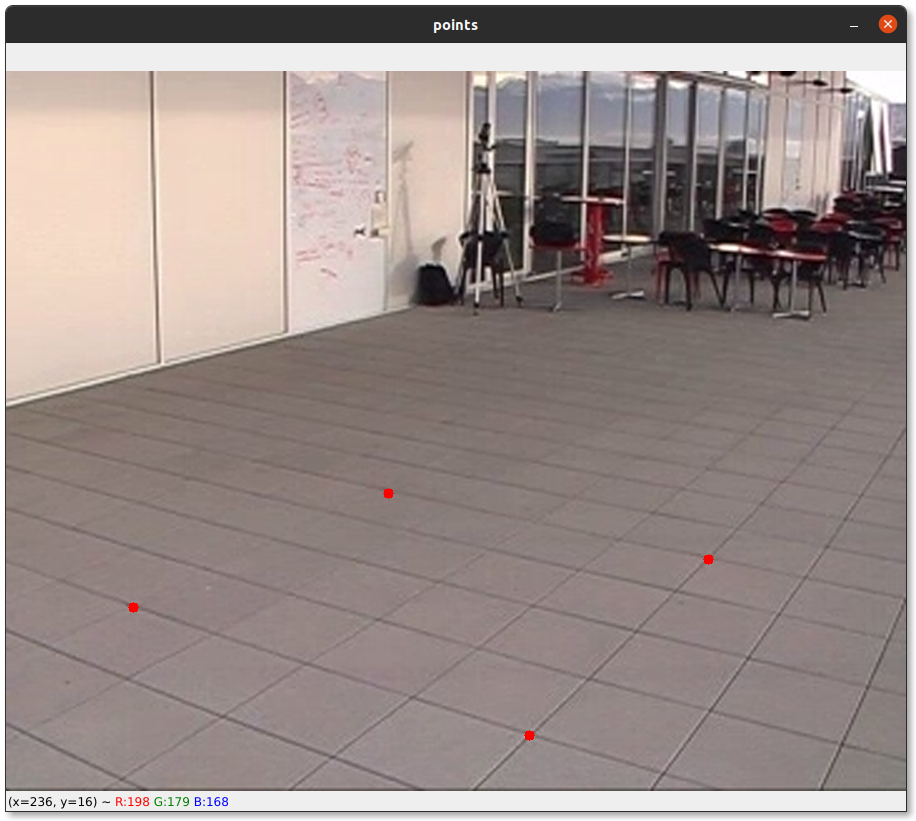
\includegraphics[width=10cm]{images/calibration1.png}
    \caption{Калибровка. Выбираем 4 точки квадрата на изображении}
    \label{<label>}
\end{figure}

Далее у пользователя запрашивается желаемый масштаб и смещение. Преобразования производятся при помощи матрицы гомографии.

Для получения матрицы используется метод OpenCV getPerspectiveTransform. В качестве параметров он принимает 4 координаты из входного и выходного изображения. Далее при помощи полученных значений кадр преобразуется в ''вид сверху'', а также с их помощью вычисляются  расстояния между людьми.


\begin{figure}[H]
    \centering
    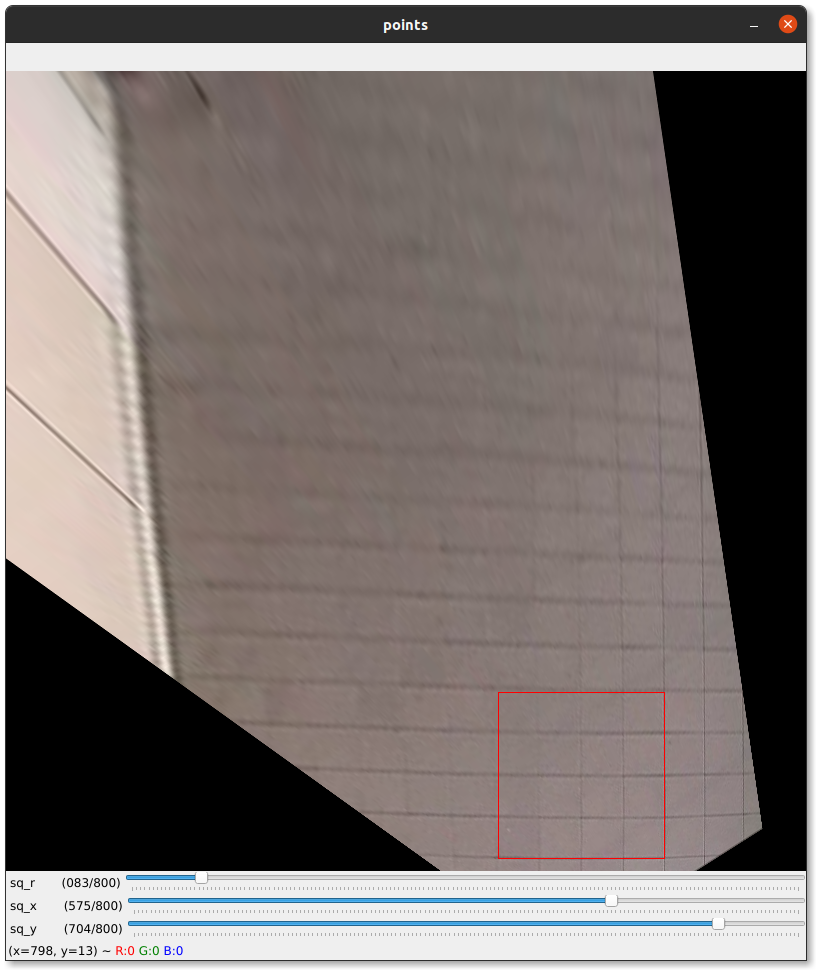
\includegraphics[width=10cm]{images/calibration2.png}
    \caption{Калибровка. Выбираем желаемый масштаб и смещение}
    \label{<label>}
\end{figure}


\section{Обнаружение людей}

Для обнаружения на изображении людей используется система распознавания YOLO. Мы используем уже обученную модель. Нейронная сеть обучалась на датасете Common Object in Context (COCO), который включает 80 категорий объектов, в том числе и людей.

%Модель глубоких сверточных нейронных сетей - это простая и эффективная модель для обнаружения объектов. Эта модель рассматривает регион, который содержит только класс "Человек", и отбрасывает регионы, которые, скорее всего, не содержат никаких объектов. Этот процесс выделения регионов, которые содержат только объекты, называется "Предложения регионов". Регионы, предсказанные с помощью предложения регионов, могут быть разного размера и перекрываться с другими регионами. Поэтому для игнорирования границ, окружающих перекрывающийся регион, в зависимости от показателя Intersection Over Union (IOU) используется максимальное неподавление.


 Мы передаем на вход изображение, а на выходе получаем координаты прямоугольников вокруг объектов, их класс и вероятность принадлежности к нему. 


\section{Вычисление расстояния}

По полученным координатам прямоугольников найдем координаты центральной точки на нижней грани. При помощи матрицы преобразования перспективы, отображаем координаты этих точек на плоскость (вид сверху).

\begin{figure}[H]
    \centering
    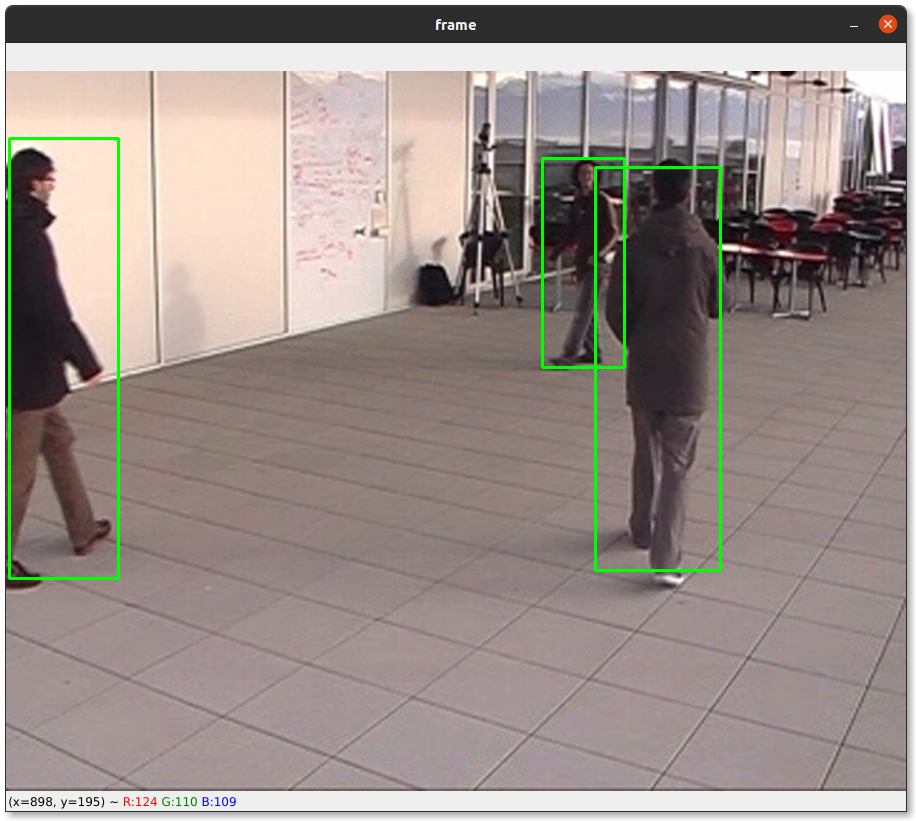
\includegraphics[width=10cm]{images/safe1.png}
    \caption{Зеленым отмечены люди на безопасной дистанции друг от друга}
    \label{<label>}
\end{figure}

Далее перебираем все возможные пары точек и вычисляем для них евклидово расстояние по проекции. Если расстояние меньше определенного значения, помечаем координату.

\begin{figure}[H]
    \centering
    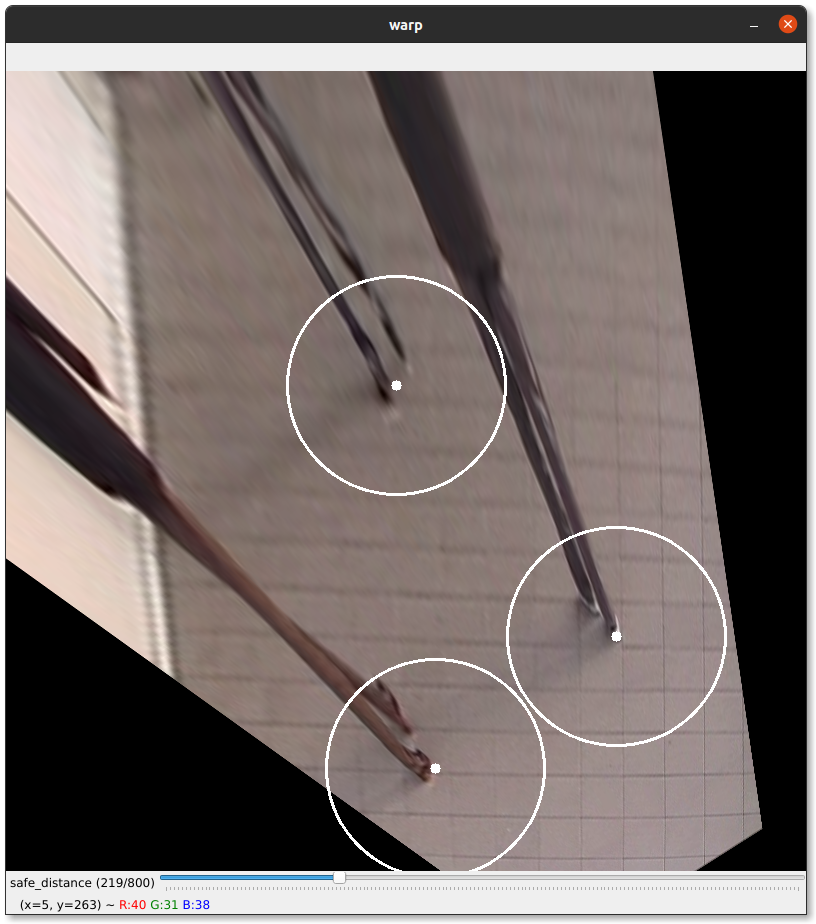
\includegraphics[width=10cm]{images/safe2.png}
    \caption{Вид сверху}
    \label{<label>}
\end{figure}

Рисуем на виде сверху окружности соответствующие безопасной дистанции, а на основном изображении, в зависимости от расстояния до других людей, рамку вокруг человека зеленого или красного цвета.

\begin{figure}[H]
    \centering
    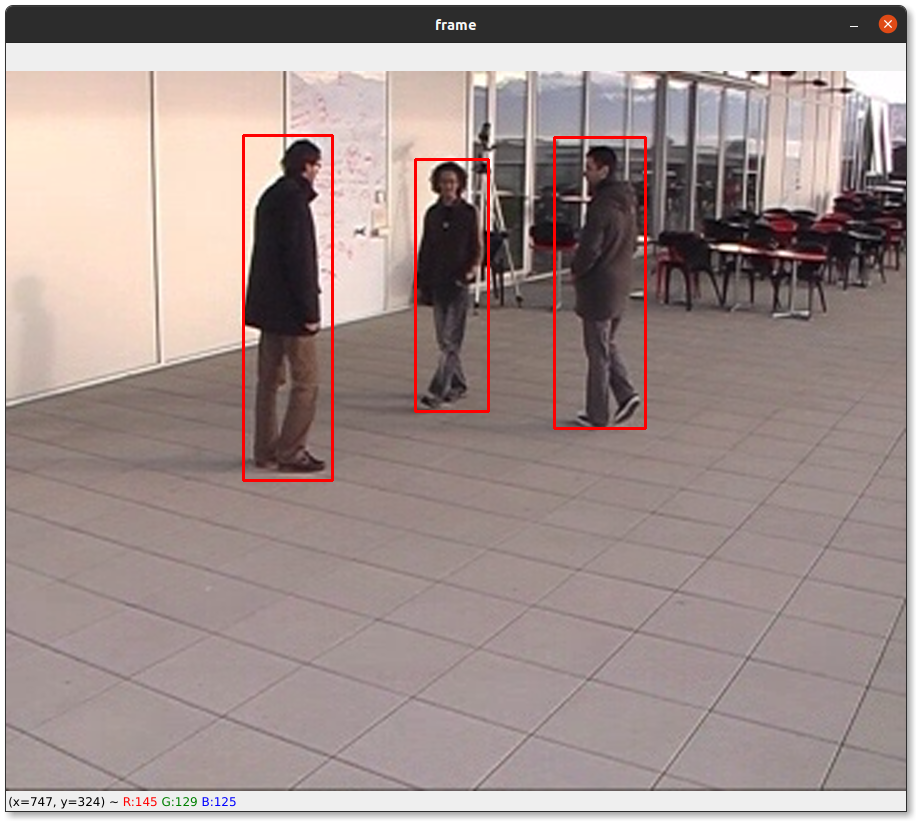
\includegraphics[width=10cm]{images/danger1.png}
    \caption{Красным отмечены люди, нарушающие социальную дистанцию}
    \label{<label>}
\end{figure}

\begin{figure}[H]
    \centering
    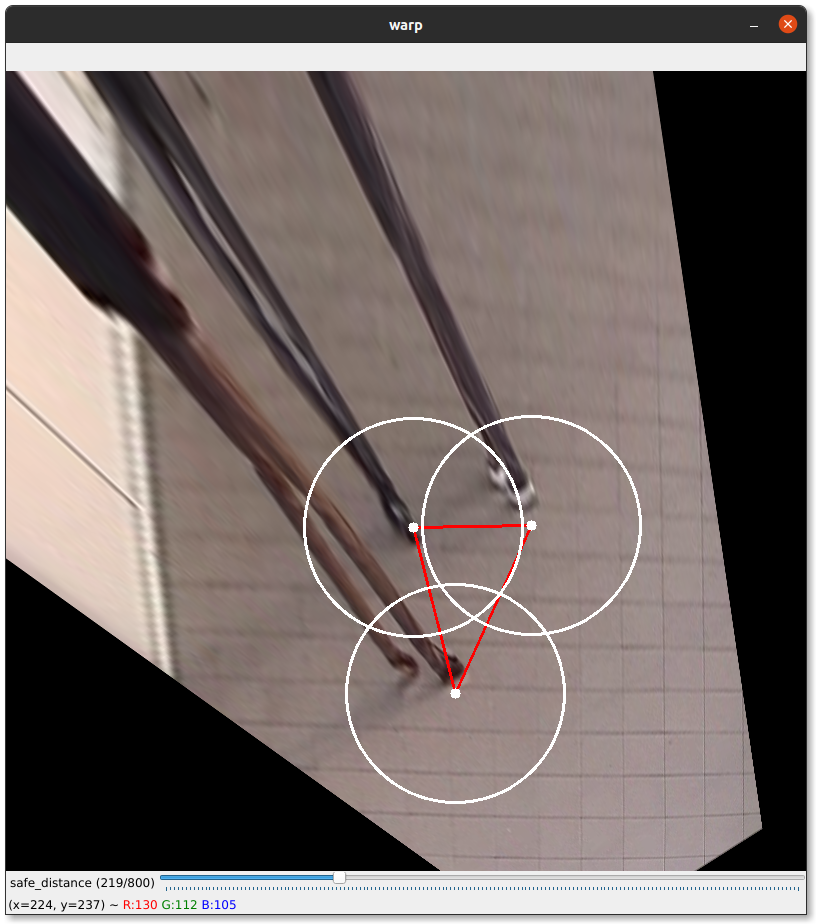
\includegraphics[width=10cm]{images/danger2.png}
    \caption{Вид сверху}
    \label{<label>}
\end{figure}
